\documentclass[lettersize,journal]{IEEEtran}
\usepackage{amsmath,amsfonts}
\usepackage{algorithmic}
\usepackage{algorithm}
\usepackage{array}
\usepackage[caption=false,font=normalsize,labelfont=sf,textfont=sf]{subfig}
\usepackage{textcomp}
\usepackage{stfloats}
\usepackage{url}
\usepackage{multicol}
\usepackage{multirow}
\usepackage{verbatim}
\usepackage[utf8]{inputenc}
\usepackage{graphicx}
\usepackage{cite}
\hyphenation{op-tical net-works semi-conduc-tor IEEE-Xplore}
% updated with editorial comments 8/9/2021

\begin{document}

\title{Radar System for Cardiopulmonary Sensing}

\author{Julio Sebastian Diaz León (judiazl@unal.edu.co)\\Omar Ferney Alvarez Herrera (oalvarezh@unal.edu.co) \\ Esteban Ladino Fajardo (eladinof@unal.edu.co) \\Sergio Andrés Lozano Avila (sealozanoa@unal.edu.co)}
        % <-this % stops a space

% The paper headers
\markboth{Radar Systems - Proyect Proposal - October 2023}%
{Shell \MakeLowercase{\textit{et al.}}: A Sample Article Using IEEEtran.cls for IEEE Journals}

%\IEEEpubid{0000--0000/00\$00.00~\copyright~2021 IEEE}
% Remember, if you use this you must call \IEEEpubidadjcol in the second
% column for its text to clear the IEEEpubid mark.

\maketitle

\begin{abstract}
In biomedical industry, there have been some explorations as radar technologies are concerned. One of those applications involves monitoring vital signs. This document shows problem statement and proposed solution for a radar system intended to measure heartbeat and respiration rate given a list of specifications which have to be met in order to ensure its best performance. related work on this topic is included as well as an action plan to be executed. 
\end{abstract}

\begin{IEEEkeywords}
Cardiology, Electronic healthcare, Health and safety, Pulmonology, Radar antennas, Radar detection, Radar measurements, Radar signal processing, Wearable Health Monitoring Systems.
\end{IEEEkeywords}


\section{Interest of the system developed, applications and previous works}


Radar systems are a widely recognized technology in constant development across various fields, including healthcare. Specifically, for cardiopulmonary sensing, it represents a technological innovation with the potential to revolutionize medical monitoring and patient care in various healthcare settings. Its development has generated significant interest both within the medical community and the technology industry, owing to its potential applications and its capacity to enhance healthcare.\\


The primary focus of the developed system lies in its non-invasive capability to detect and monitor vital signs (as cited in the presentation by Julio/Esteban), such as heart rate and respiration, using radar waves. This eliminates the need for sensors or devices requiring direct skin contact, enabling continuous and precise patient monitoring. This is particularly beneficial in critical environments such as intensive care units, for example, in the case of burn patients (as cited in the presentation by Julio/Esteban).\\

The applications of this system are diverse, spanning from healthcare in hospitals to remote patient monitoring in homes, leveraging high-speed internet connections via fiber optics and even 5G, integrating IoT monitoring systems for data transmission to healthcare centers and specialists. Moreover, it can be employed for early detection of abnormal cardiac and respiratory events, which is crucial for preventive care and the development of public health policies focused on prevention.\\

There is a substantial body of articles, conferences, and reviews that demonstrate a keen interest in the use of this technology and show significant progress in the field. Prototypes have been implemented with humans, yielding tangible and consistent results when compared to well-established methods, such as electrocardiography, sensors, and even smartwatches equipped with optical sensors.\\

Returning to an initial article that refers to algorithms for detecting vital signs, we can mention "Ultra-wide band impulse radar for life detection using wavelet packet decomposition," published in the Journal Physical Communication by ScienceDirect. This article presents an improved algorithm for life detection using ultra-wide band impulse radar (UWB) through walls. Although in our project development, we aim for scenarios without obstacles in transmission or reception, this condition is worth considering. It contributes to the state of the art in the field, as it can detect cardiac and respiratory movements. The algorithm analyzes variations in collected pulses, which are influenced by factors such as time of arrival (TOA) between the UWB radar and the human subject, calculated through wavelet packet decomposition. Frequencies of human cardiac and respiratory movements are collected through a variable time window (VTW).\\

A second article to consider is presented at the IEEE Radio and Wireless Symposium (RWS) 2023, titled "Accurate Heart Beat Detection with Doppler Radar using Bidirectional GRU Network." This article offers insights into the use of neural networks for obtaining vital signs through a Doppler radar, potentially making it a valuable choice for our project. It also considers continuous wave (CW) radar, where the signal processing involves a four-stage method: baseband signal collection, Butterworth filtering, noise elimination, and the application of a neural network model.\\


A third document worth mentioning is "Super-Regenerative Oscillator Based High-Sensitivity Radar Architecture for Motion Sensing and Vital Sign Detection," published in IEEE Transactions on Microwave Theory and Techniques. Its major contribution to the state of the art lies in establishing a functional architecture for radar system implementation, incorporating a component called the super-regenerative oscillator (SRO) and a 2.32 GHz patch antenna. As a complementary aspect to the project's development, it addresses the absence of RF signal generators, offering an alternative that doesn't rely on software-defined radios like USRP, potentially reducing costs.\\

With a radar system is possible measurements several patient vital signs and it is necessary to identify other sources as human movements \cite{f.kraiemDopplerRadarArchitecture2019}. Other contactless methods as thermal imagining, infrared thermography equipment, and video imaging have problems in implementation to the cost or physics requirements \cite{f.kraiemDopplerRadarArchitecture2019}. The radars can also be used to search for survivors in disasters and control security areas \cite{f.kraiemDopplerRadarArchitecture2019}.        



\section{Problem statement and specifications}

The main objective of this project is to develop a system capable of measuring heartbeat and respiration rates. In order to assess its quality, there are some specifications that radar system must fulfil as follows:

\begin{itemize}
    \item System's spectrum usage must comply applicable law.
    \item Measurement distance from subject must be from 0 to 2 meters.
    \item Real-time operation, heart rate and respiration rate display at most ten seconds after the positioning of the subject in front of the radar.
    \item System must include indication of the presence or absence of a subject.
    \item Maximum measurement error: 20\% for both heart and respiratory rates.
    \item False alarm rate of subject presence less than 20\%.
    \item Detection rate of subject presence 70\%.
\end{itemize}



\section{Project Planning}

In this section, planning method is explained including list of activities, a schedule for project development and a state of advance of ongoing tasks. 

\section{List Of Activities}

Below list of activities with its respective Gantt Chart:


\section{Approximate budget including student time}

Below Budget analysis

\begin{table*}[]
\centering
\caption{Budget Analysis}
\label{tab:budget}
\begin{tabular}{|c|c|c|c|c|r|r|}
\hline
Item &
  Concept &
  Reference &
  Brand &
  Quantity &
  \multicolumn{1}{c|}{Cost (USD)} &
  \multicolumn{1}{c|}{Total (USD)} \\ \hline
\multirow{5}{*}{Antenna} &
  SMA   Interconnect &
  086-9KM+ &
  Minicircuits &
  2 &
  109,66 &
  219,32 \\ \cline{2-7} 
                         & SMA   Connector     & 471-SMA        & LPRS        & 2 & 1,46           & 2,92      \\ \cline{2-7} 
                         & Simulator           & Student        & Ansys       & 1 & Free   license & 0         \\ \cline{2-7} 
                         & PCBs                & FR4            & Vector      & 2 & 17,88          & 35,76     \\ \cline{2-7} 
                         & CNC   prototype     & -              & PCway       & 5 & 12,00          & 12,00     \\ \hline
USRP &
  \multicolumn{1}{l|}{Software   Radio Define} &
  \multicolumn{1}{l|}{B200mini} &
  \multicolumn{1}{l|}{National instruments} &
  1 &
  1.323,00 &
  1.323,00 \\ \hline
Work &
  \multicolumn{1}{l|}{Development} &
  \multicolumn{1}{l|}{-} &
  \multicolumn{1}{l|}{RF engineer} &
  4 &
  3.500,00 &
  14.000,00 \\ \hline
Laptop &
  \multicolumn{1}{l|}{Laptop} &
  \multicolumn{1}{l|}{Vivo Book} &
  \multicolumn{1}{l|}{Asus} &
  1 &
  1.000,00 &
  1.000,00 \\ \hline
\multirow{4}{*}{Phantom} & Globe   and syringe & -              & Nipro       & 1 & 2,00           & 2,00      \\ \cline{2-7} 
                         & Audio   cable       & -              & -           & 1 & 1,00           & 1,00      \\ \cline{2-7} 
                         & 3.5mm   plug        & -              & -           & 1 & 2,00           & 2,00      \\ \cline{2-7} 
                         & Speaker   1W 8 Ohm  & CMS-2039-128SP & CUI Devices & 1 & 2,34           & 2,34      \\ \hline
Software                 & Control RF software & RF             & GNUradio    & 1 & Free license   & 0         \\ \hline
Misc                     &                     &                &             & 1 & 4.980,10       & 4.980,10  \\ \hline
Total                    &                     &                &             &   &                & 21.580,44 \\ \hline
\end{tabular}
\end{table*}

\section{Validation testbed}

proposal of a hardware device that simulates a person with representative size, and heart/respiration rates.

\section{Detailed definition of the protocol followed to evaluate all the specifications}



\section{Preliminary results}

Description of any design/simulation results obtained in the development of the project.

\subsection{Design}

Patch antenna is designed according to Figure \ref{fig:AntThe} and Equations \eqref{eq:des_w}, \eqref{eq:e_eff}, \eqref{eq:delta_L_h}, \eqref{eq:delta_L}, \eqref{eq:L_TM}, \eqref{eq:L_eff} y \eqref{eq:lambda_0}. Values given are:

\begin{itemize}
\item  $\epsilon_r=4.4$
\item $f_r=5.8 \; [GHz]$
\item $h=60 \; [mm]$

\end{itemize}


\begin{figure}[H]
\centering
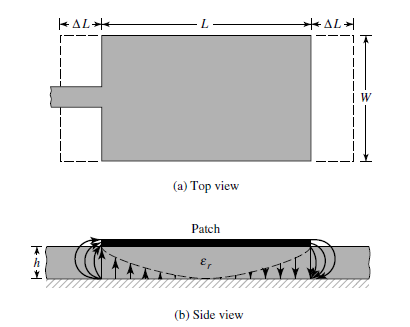
\includegraphics[width=1\linewidth]{figs/AntThe.png}
\caption{Patch antenna parameters. \cite{balanisAntennaTheoryAnalysis2005}}
\label{fig:AntThe}
\end{figure}



\begin{align}
\label{eq:des_w}
w &=\frac{v_0}{2 f_r} \sqrt[2]{\frac{2}{\epsilon_r+1}} \\ \nonumber
 &= \frac{30}{2 \times 5.8}\sqrt[2]{\frac{2}{4.4+1}} \\ \nonumber 
 & =1.573 \; [cm]
\end{align}


\begin{align}
    \label{eq:e_eff}
    \epsilon_{reff} &= \frac{\epsilon_r+1}{2}+\frac{\epsilon_r-1}{2}\left[1+12\left(\frac{h}{w}\right)\right]^{-\frac{1}{2}} \\ \nonumber
    &=\frac{4.4+1}{2}+\frac{4.4-1}{2}\ast\left[1+12\left(\frac{0.1524}{1.573}\right)\right]^{-\frac{1}{2}} \\ \nonumber
    &=3.856
\end{align}

\begin{align}
    \label{eq:delta_L_h}
    \frac{\Delta L}{h} &= 0.412 \left(\frac{\left(\epsilon_{reff}+0.3\right)\left(\frac{w}{h}+0.264\right)}{\left(\epsilon_{reff}-0.258\right)\left(\frac{w}{h}+0.8\right)} \right) \\  \nonumber 
\end{align}

\begin{align}
    \label{eq:delta_L}
    \Delta L &= 0.412h \left( \frac{\left(3.856+0.3\right)\left(\frac{1.573}{0.1524}+0.264\right)}{\left(3.856-0.258\right)\left(\frac{1.573}{0.1524}+0.8\right)} \right) \\ \nonumber
    &= 0.06903 \; [cm]
\end{align}

\begin{align}
    \label{eq:L_TM}
    L_{TM010}&=\frac{\lambda_d}{2}-2 \Delta L \\ \nonumber
    &=2.572 \; [cm]
\end{align}

\begin{align}
    \label{eq:L_eff}
    L_{eff}&=L+2 \Delta L \\ \nonumber
    &= 2.586+2\left(0.06903\right)=2.6\approx\frac{\lambda_d}{2}
\end{align}

\begin{align}
    \label{eq:lambda_0}
    \lambda_0&=\frac{v_0}{f} \\ \nonumber
    &=51.72 \; [mm]
\end{align}

\subsection{Results}


Frequency and Bandwidth antenna is according to resolution 115 of 23 March 2020  by Agencia Nacional del Espectro (ANE) \cite{ANERes105}. This specific that from 5725 to 5875 MHz  is part of ISM bands.   

\section{Description of the challenges foreseen for the completion of the project and how these will be faced.}








\begin{thebibliography}{1}
\bibliographystyle{IEEEtran}

\bibitem{kakouche}
I. Kakouche, A. Maali, M. N. El Korso, A. Mesloub, M. S. Azzaz, "Fast and cost-effective method for non-contact respiration rate tracking using UWB impulse radar," Sensors and Actuators A: Physical, vol. 329, pp. 112814, 2021, \url{doi: 10.1016/j.sna.2021.112814.}

\bibitem{ane_free_spectrum}
Agencia Nacional del Espectro (2023, October 16). Gestión técnica. [Online]. Available: \url{https://www.ane.gov.co/SitePages/Gestión%20técnica/index.aspx?p=23}

\bibitem{f.kraiemDopplerRadarArchitecture2019} 
F. Kraiem, M. Dhieb, M. Ketata, H. Ghariani, y M. Lahiani, Doppler Radar Architecture for Vital Signal Detection, en 2019 IEEE International Conference on Design \& Test of Integrated Micro \& Nano-Systems (DTS), may 2019, pp. 1-5. doi: \url{10.1109/DTSS.2019.8915187.}

\bibitem{ANERes105} Agencia Nacional del Espectro (ANE), Resolución No. 105 de 27 de marzo de 2020, ``Por medio de la cual se actualiza el Cuadro Nacional de Atribución de Bandas de Frecuencias''. República de Colombia, 2020.


\bibitem{balanisAntennaTheoryAnalysis2005} C. A. Balanis, Antenna theory: analysis and design, 3rd ed. Hoboken, NJ: John Wiley, 2005.


\end{thebibliography}



\end{document}

